\section{Methods}

\subsection{Model Architecture}

MelanomaNet uses EfficientNetV2-M \cite{tan2021efficientnetv2} as the backbone
feature extractor. EfficientNetV2 is trained with a combination of
training-aware neural architecture search and progressive learning, which the
original authors report as improving both training speed and parameter
efficiency. The medium variant has 54 million parameters and produces a
1280-dimensional feature vector, a capacity that fits the dataset size without
the cost of the large variant.

Images are processed at $384\times384$ rather than the $224\times224$ common in
general image classification. The higher resolution retains the fine pigment
and border detail that dermoscopy depends on. The classification head applies
global average pooling, dropout (rate 0.3), and a linear layer. ISIC 2019
defines nine diagnostic categories, so the layer produces nine logits; however,
the ninth ``unknown'' (UNK) category contains no labelled images, so in practice
the model learns and is evaluated on the eight populated classes: Melanoma
(MEL), Nevus (NV), Basal Cell Carcinoma (BCC), Actinic Keratosis (AK), Benign
Keratosis (BKL), Dermatofibroma (DF), Vascular lesion (VASC), and Squamous Cell
Carcinoma (SCC). Because UNK never appears in the ground truth, its logit is
never reinforced during training and it is omitted from all reported metrics.

Figure \ref{fig:architecture} illustrates the complete system architecture,
showing how the classification pipeline integrates with four explainability
modules that operate on different levels of the model's representation.

\begin{figure*}[t]
    \centering
    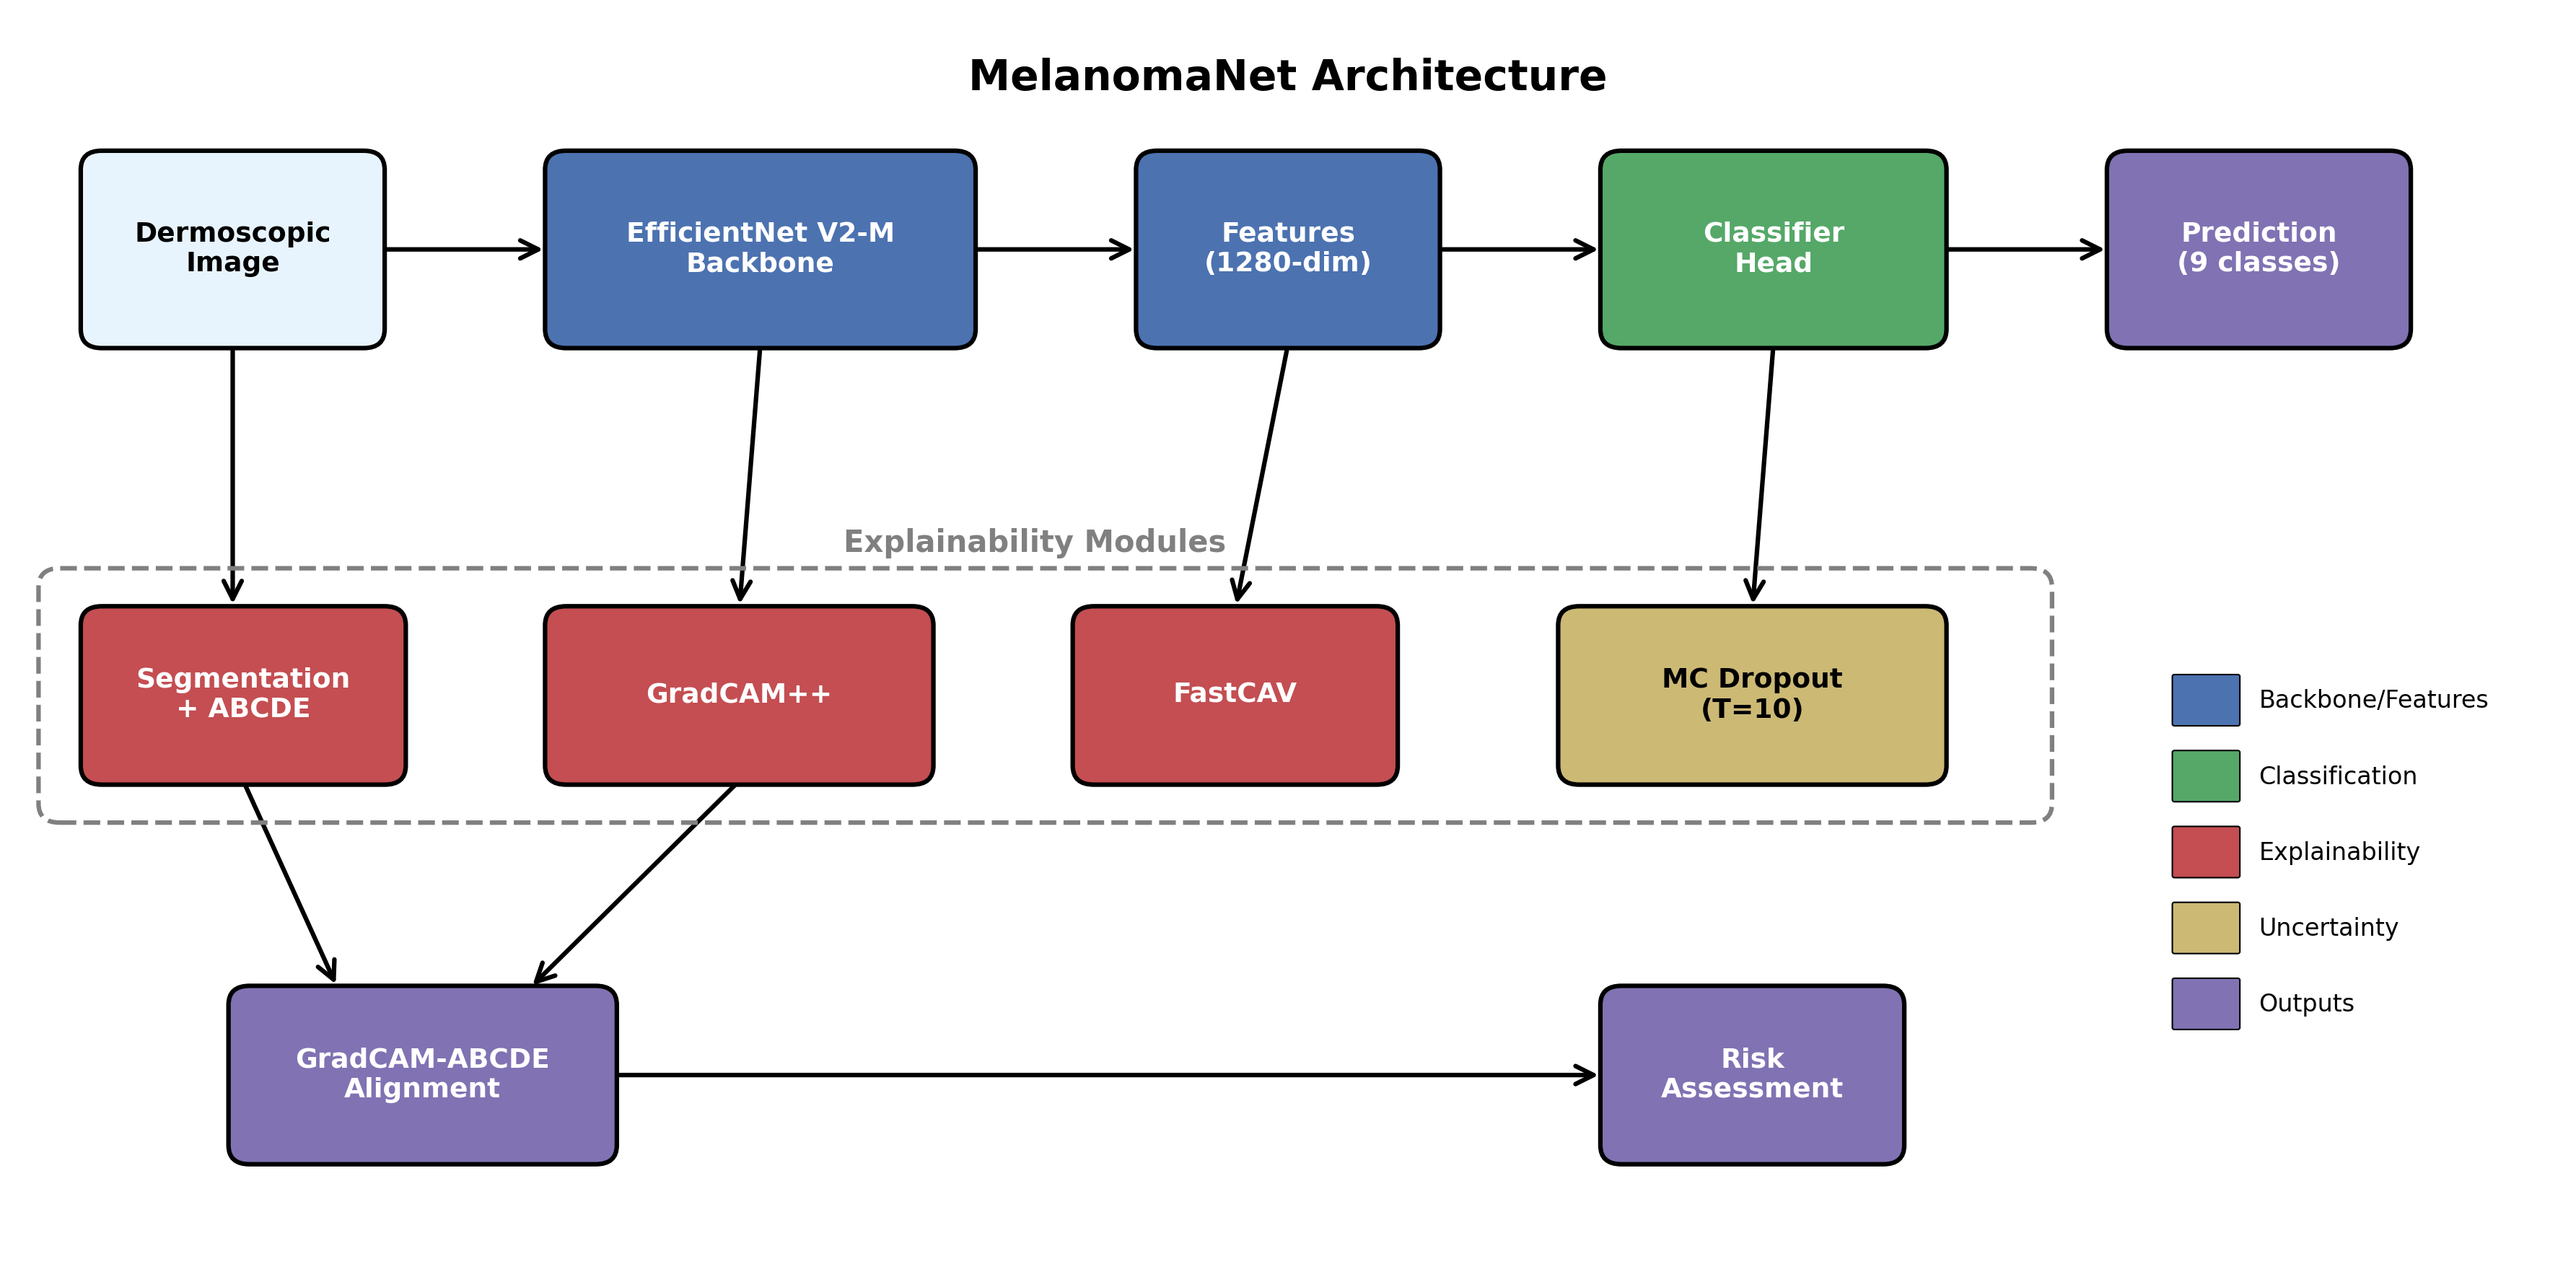
\includegraphics[width=0.95\textwidth]{figures/architecture.png}
    \caption{MelanomaNet system architecture. The main classification pipeline
        (top) processes dermoscopic images through EfficientNet V2-M to produce
        predictions across 8 classes. Four explainability modules (bottom, dashed box)
        provide complementary interpretations: ABCDE clinical criteria from image
        segmentation, GradCAM++ attention from feature maps, SGD-CAV concept scores
        from extracted features, and MC Dropout uncertainty estimates from stochastic
        forward passes. The GradCAM-ABCDE alignment module validates correspondence
        between model attention and clinical features.}
    \label{fig:architecture}
\end{figure*}

\subsection{Training Configuration}
\label{sec:methods-training}

We train using weighted cross-entropy loss to address significant class
imbalance in the dataset, with class weights inversely proportional to class
frequencies. Optimization employs AdamW with initial learning rate $10^{-4}$,
weight decay $10^{-4}$, and cosine annealing schedule over 100 epochs. Mixed
precision training accelerates computation while maintaining numerical
stability. Data augmentation includes random horizontal and vertical flips,
rotation ($\pm20^\circ$), affine transformations (translation 10\%, scale
0.9--1.1), and color jittering (brightness, contrast, saturation 0.2, hue 0.1).

\subsection{GradCAM++ Attention Visualization}

We employ GradCAM++ \cite{chattopadhay2018grad} to visualize which image
regions most influence the model's predictions. GradCAM++ improves upon
GradCAM by computing pixel-wise importance weights for feature map
activations, providing better localization for multiple objects and sharper
attention maps. The method computes gradients of the predicted class score
with respect to the final convolutional layer's feature maps, then weights
and combines these activations to produce a class-discriminative heatmap.
The resulting visualization is upsampled to input resolution and overlaid
on the original image, allowing clinicians to verify that the model attends
to the lesion rather than spurious background features.

\subsection{ABCDE Clinical Criterion Analysis}

We implement automated extraction of ABCDE features to bridge model
predictions with clinical reasoning:

\textbf{Lesion Segmentation}: We extract lesion masks using Otsu's
thresholding with morphological refinement. Connected component analysis
removes small artifacts, and hole-filling produces robust binary masks.

\textbf{Asymmetry (A)}: We compare lesion halves along horizontal and
vertical axes through the centroid. The asymmetry score quantifies the
non-overlapping area between reflected halves, normalized to $[0,1]$.

\textbf{Border Irregularity (B)}: We analyze contour properties including
compactness (perimeter$^2$/area) and vertex count from polygon approximation.
Higher scores indicate more irregular borders.

\textbf{Color Variation (C)}: K-means clustering ($k=6$) identifies distinct
colors within the lesion. We count colors exceeding 5\% coverage and compute
color standard deviation as a variation score.

\textbf{Diameter (D)}: We compute the minimum enclosing circle and bounding
box diagonal, reporting the maximum extent in pixels.

\textbf{Risk Stratification}: A composite risk score sums binary flags from
each criterion (thresholds: asymmetry $>0.3$, border $>0.4$, colors $>3$,
diameter $>114$ pixels). Scores $\geq3$ indicate high risk, $\geq2$ medium
risk, and $<2$ low risk.

\subsection{GradCAM-ABCDE Alignment}

To validate that model attention corresponds to clinically relevant features,
we compute alignment metrics between GradCAM heatmaps and ABCDE analysis:

\begin{equation}
    \text{Alignment}_{\text{border}} = \frac{\sum_{i,j} M_{\text{border}}(i,j)
        \cdot H(i,j)}{\sum_{i,j} M_{\text{border}}(i,j)}
\end{equation}

where $M_{\text{border}}$ is a dilated border mask and $H$ is the normalized
attention heatmap. Similar metrics quantify attention overlap with the
overall lesion region.

\subsection{Concept Activation Vectors}

We explain predictions in terms of clinical concepts using concept activation
vectors, following TCAV \cite{kim2018interpretability}. To keep training cheap
we fit each concept classifier with stochastic gradient descent rather than the
support-vector solver used in the original work; we refer to this variant as
SGD-CAV to distinguish it from the separately proposed FastCAV method of
Schmalwasser et al.\ \cite{schmalwasser2025fastcav}, which accelerates the same
computation in a different way. For each clinical concept (asymmetry, irregular border,
multiple colours, large diameter) we collect concept-positive and
concept-negative example images, extract their 1280-dimensional features, and
train a linear classifier to separate them. The concept activation vector (CAV)
$v_c$ is the unit normal to the resulting decision boundary.

For a given image we report the directional sensitivity of the prediction to the
concept, computed as the projection of the (standardised) feature vector onto
$v_c$. The score is signed and unbounded: a positive value indicates that the
concept is expressed in a way that supports the predicted class, a negative
value indicates the opposite, and the magnitude reflects the strength of the
association. This is a per-image sensitivity rather than the aggregate TCAV
score of \cite{kim2018interpretability}, which is instead the fraction of a set
of images with a positive directional derivative.

\subsection{MC Dropout Uncertainty Quantification}

We employ Monte Carlo Dropout \cite{gal2016dropout} with $T=10$ stochastic
forward passes to estimate uncertainty. By keeping dropout active during
inference, each forward pass samples from an approximate posterior
distribution over model weights, enabling Bayesian uncertainty estimation
without explicit probabilistic modeling. For each input, we compute three
complementary uncertainty measures:

\textbf{Predictive Uncertainty} captures total model uncertainty through
the entropy of averaged predictions:
\begin{equation}
    H[\bar{p}] = -\sum_c \bar{p}_c \log \bar{p}_c, \quad
    \bar{p} = \frac{1}{T}\sum_{t=1}^T p_t
\end{equation}
where $p_t$ is the softmax output from forward pass $t$, $\bar{p}$ is the
mean prediction across all $T$ passes, and $c$ indexes over classes. Higher
entropy indicates the model is uncertain about which class to predict.

\textbf{Epistemic Uncertainty} measures model uncertainty arising from
limited training data:
\begin{equation}
    \text{Var}[p] = \frac{1}{T}\sum_{t=1}^T (p_t - \bar{p})^2
\end{equation}
This variance across stochastic forward passes quantifies how much the
model's predictions fluctuate when different subsets of neurons are dropped.
High epistemic uncertainty suggests the model lacks sufficient training
examples similar to the input, and can be reduced with more data.

\textbf{Aleatoric Uncertainty} captures inherent data noise that cannot
be reduced:
\begin{equation}
    \frac{1}{T}\sum_{t=1}^T H[p_t]
\end{equation}
This averages the entropy of individual predictions, reflecting uncertainty
due to ambiguous or overlapping features in the input itself. Unlike
epistemic uncertainty, aleatoric uncertainty persists regardless of
training data quantity.

Predictions with predictive uncertainty exceeding threshold 0.5 are flagged
as unreliable, prompting clinical review. This decomposition allows
clinicians to understand whether uncertainty stems from model limitations
(epistemic) or inherent case ambiguity (aleatoric).
